 \chapter{Resultados}
\label{cap:resultados}

\section{Introdução}
Este capítulo apresenta os resultados obtidos com o desenvolvimento do site e do ambiente virtual, correlacionando-os diretamente aos objetivos estabelecidos no início deste trabalho. Demonstra-se como cada objetivo foi atendido, com destaque para as melhorias implementadas em relação ao estado anterior do site e a criação de um ambiente virtual \gls{3d} interativo para a divulgação e preservação da arte rupestre.

\section{Objetivo Geral}
O objetivo geral deste trabalho é desenvolver uma plataforma web e um ambiente virtual \gls{3d} que permitam a preservação, divulgação e o acesso à arte rupestre da Lapa da Pedra. Esse projeto busca oferecer uma experiência interativa para educadores, pesquisadores e o público em geral, promovendo a conscientização sobre a importância desses registros culturais. Esse objetivo foi atingido por meio da entrega de:
\begin{itemize}
    \item Um novo site moderno, acessível e responsivo, que organiza as informações de forma clara e permite fácil navegação.
    \item Um ambiente virtual interativo que possibilita a visualização detalhada das pinturas rupestres e oferece uma experiência imersiva aos usuários.
    \item Funcionalidades que tornam o site útil para educadores, pesquisadores e o público geral, como galeria de imagens, acesso a modelos \gls{3d} e artigos publicados.
\end{itemize}

As seções a seguir detalham como os objetivos específicos foram atendidos.

\section{Objetivos Específicos}

\subsection{Análise Heurística de Usabilidade: Problemas Identificados no Site Antigo}
Um dos objetivos específicos era realizar uma análise heurística de usabilidade do antigo site "Arqueologia Formosa". Essa análise foi conduzida com base nas heurísticas de Nielsen, avaliando aspectos como navegabilidade, eficiência e consistência. Os principais problemas identificados foram:
\begin{itemize}
    \item Layout desorganizado, dificultando a localização de informações importantes.
    \item Falta de responsividade para dispositivos móveis.
    \item Ausência de funcionalidades modernas, como busca eficiente e compartilhamento em redes sociais.
\end{itemize}

Esses problemas foram utilizados como base para o planejamento do novo site, garantindo que as falhas do sistema anterior fossem corrigidas. A análise heurística também guiou a priorização das melhorias implementadas.

\subsection{Desenvolvimento de um Novo Site com Design Centrado no Usuário (\gls{ux})}
O novo site foi desenvolvido com tecnologias modernas (\textit{Next.js}, \textit{Tailwind CSS} e \textit{Sanity CMS}), priorizando uma experiência do usuário intuitiva e acessível. Os resultados alcançados incluem:
\begin{itemize}
    \item Design responsivo, otimizado para dispositivos móveis, desktops e tablets.
    \item Galeria de imagens organizada, com suporte para visualização ampliada.
    \item Modo escuro/claro, permitindo maior conforto visual.
    \item Implementação de padrões de acessibilidade conforme WCAG 2.1 (nível AA).
\end{itemize}

A Figura \ref{fig:site_homepage} apresenta a página inicial do novo site, evidenciando o layout moderno e a organização do conteúdo.

\begin{figure}[H]
    \centering
    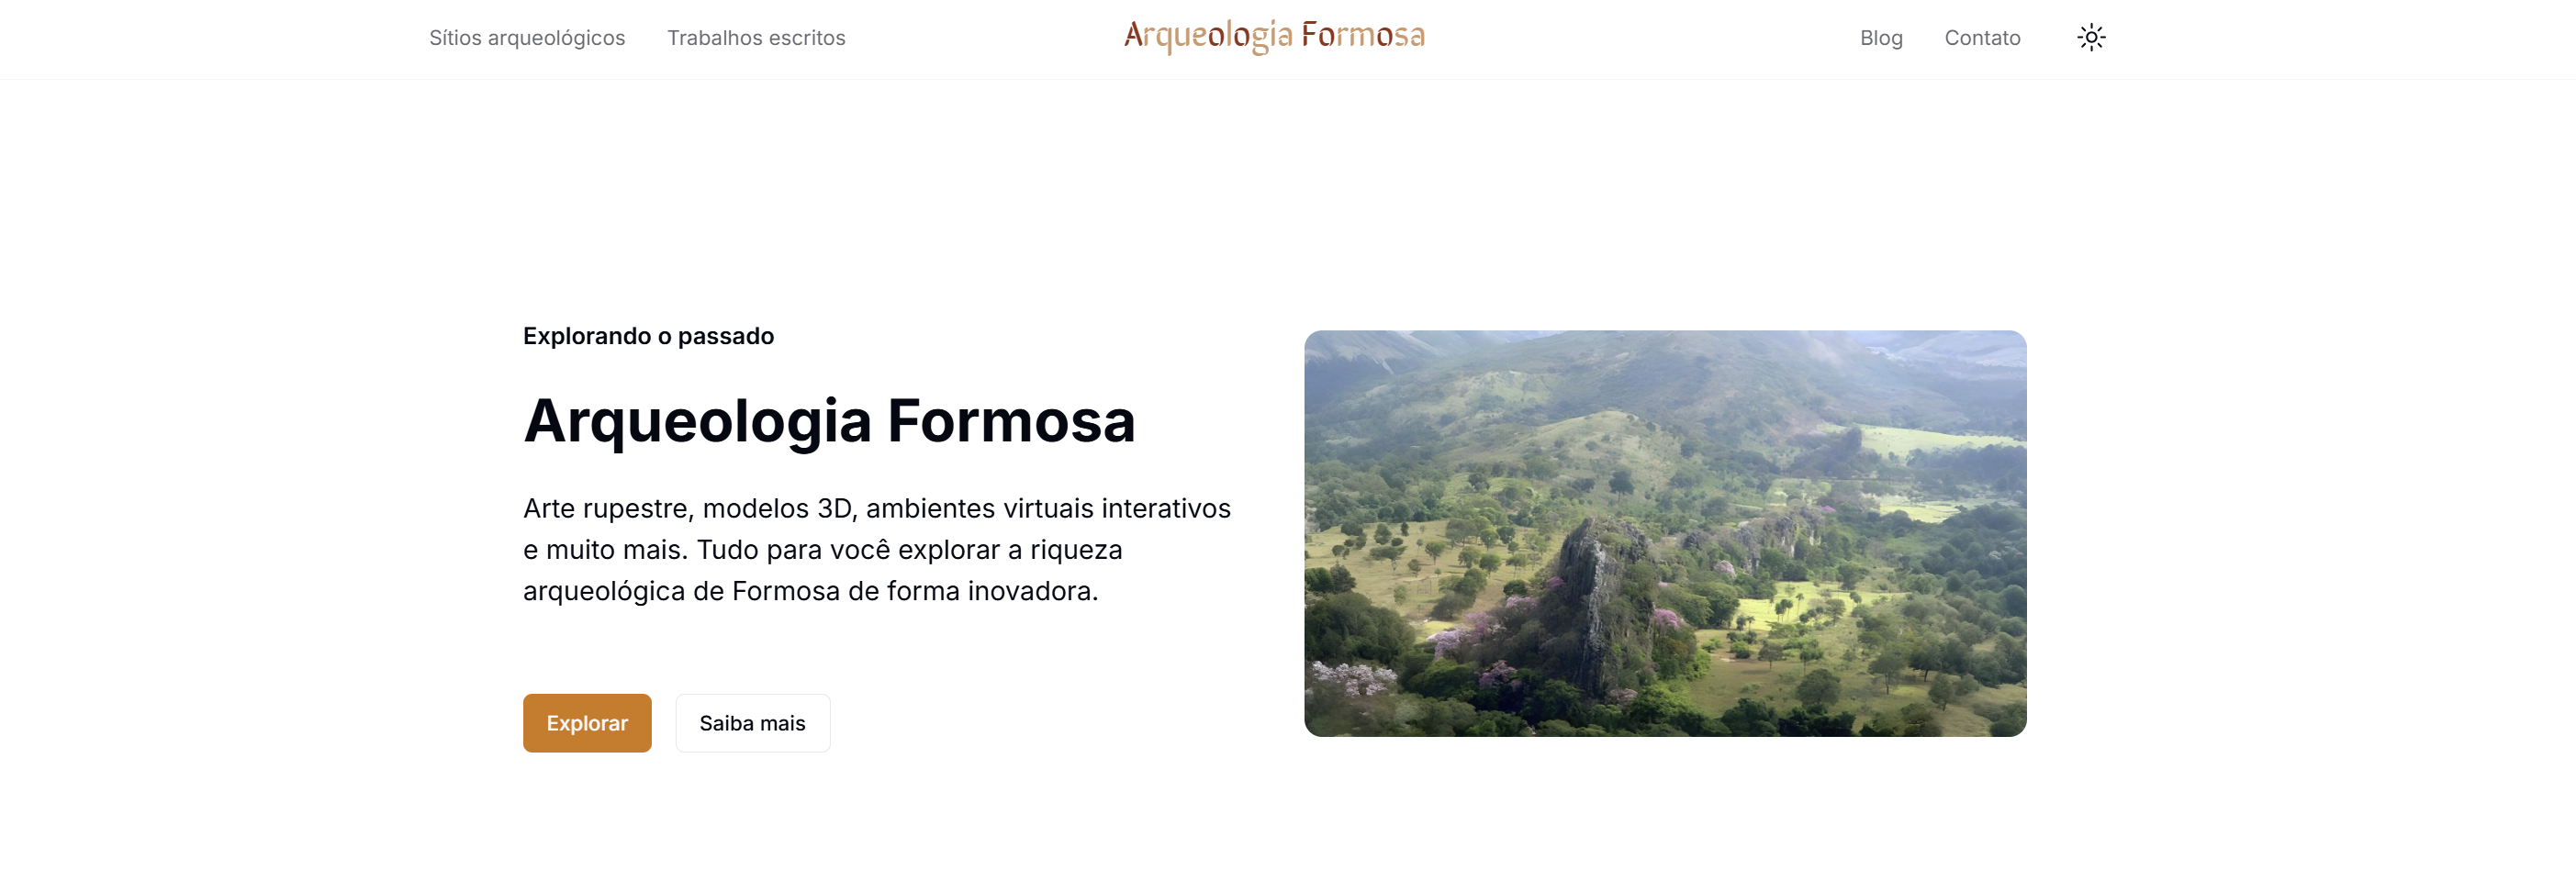
\includegraphics[height=6cm, keepaspectratio]{img/site/hero1.png}
    \caption{Página inicial do novo site "Arqueologia Formosa". \\
    \textbf{Fonte:} Elaborado pelo autor.}
    \label{fig:site_homepage}
\end{figure}

As demais páginas podem ser vista no Apêndice \ref{ap:páginas_do_site} e no site publicado na internet, acessível por meio do endereço \url{www.arqueologiaformosa.com.br}.
\subsection{Implementação de um Ambiente Virtual \gls{3d}}
Outro objetivo específico era implementar um ambiente virtual \gls{3d} que permitisse a visualização interativa da arte rupestre. Esse objetivo foi alcançado com o desenvolvimento de um ambiente imersivo na Unreal Engine, utilizando modelos \gls{3d} gerados por fotogrametria. Os resultados incluem:
\begin{itemize}
    \item Fidelidade visual dos modelos \gls{3d}, com texturas realistas das pinturas rupestres.
    \item Navegação interativa no ambiente, permitindo aos usuários explorar o sítio arqueológico.
    \item Empacotamento do ambiente virtual em um arquivo executável, disponibilizado para \textit{download} no site.
\end{itemize}

A Figura \ref{fig:virtual_environment} apresenta uma visão do ambiente virtual desenvolvido.

\begin{figure}[H]
    \centering
    % Substitua pelo caminho do arquivo de imagem
    \includegraphics[width=0.8\linewidth]{images/virtual_environment.png}
    \caption{Ambiente virtual desenvolvido na Unreal Engine.}
    \label{fig:virtual_environment}
\end{figure}


\section{Testes e Validação}

\subsection{Usabilidade}
Os testes de usabilidade foram realizados com base nas heurísticas de Nielsen. Os seguintes pontos foram avaliados:
\begin{itemize}
    \item Facilidade de navegação no site e no ambiente virtual.
    \item Eficiência na interação com a galeria de imagens e o ambiente virtual.
    \item Satisfação dos usuários com o design e as funcionalidades implementadas.
\end{itemize}


\begin{table}[H]
\centering
\caption{Resultados dos testes de usabilidade.}
\label{tab:usabilidade}
\begin{tabularx}{\textwidth}{|l|X|X|} % Ajusta a largura da tabela ao texto
\hline
\textbf{Critério Avaliado} & \textbf{Pontuação Média} & \textbf{Observações} \\ \hline
Facilidade de Navegação    & 4.7/5                   & Navegação intuitiva e bem estruturada. \\ \hline
Interação com o Conteúdo    & 4.6/5                   & Boa experiência na galeria de imagens e no ambiente virtual. \\ \hline
Design e Funcionalidades    & 4.8/5                   & Alta satisfação com o layout moderno e intuitivo. \\ \hline
\end{tabularx}
\end{table}

\subsection{Desempenho}
Os testes de desempenho foram realizados com o Google Lighthouse. Abaixo estão os principais resultados:
\begin{itemize}
    \item Tempo de carregamento médio: 2.3 segundos.
    \item Pontuação em SEO: 100/100.
    \item Responsividade: 100\% em dispositivos móveis e desktops.
\end{itemize}

\begin{figure}[H]
    \centering
    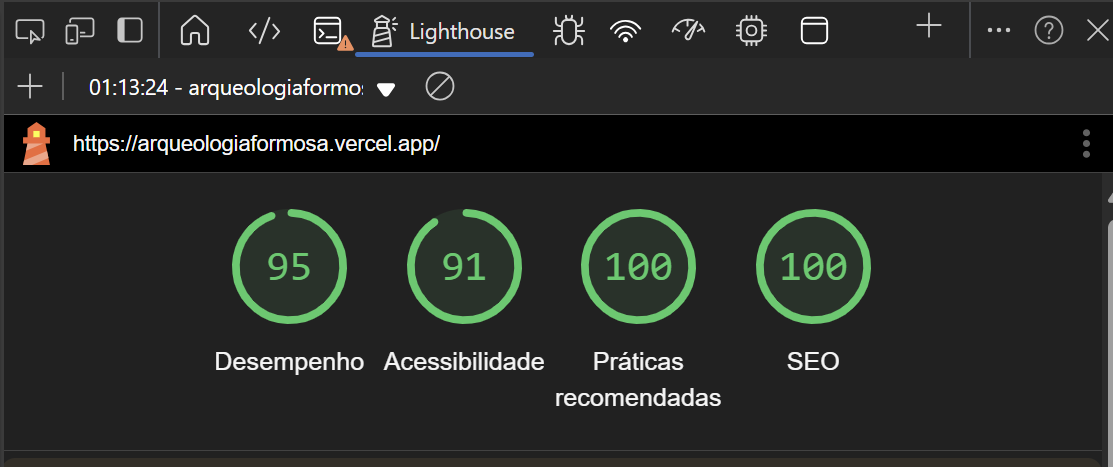
\includegraphics[height=6cm, keepaspectratio]{img/site/lighthouse_only.png}
    \caption{nálise de desempenho do site Arqueologia Formosa pela ferramenta \textit{Lighthouse}. \\
    \textbf{Fonte:} Elaborado pelo autor.}
    \label{fig:site_homepage}
\end{figure}

\subsection{Acessibilidade}
Conformidade com as diretrizes WCAG 2.1:
\begin{itemize}
    \item Contraste adequado para textos e botões.
    \item Navegação por teclado funcionando corretamente.
    \item Compatibilidade com leitores de tela.
\end{itemize}


\section{Conclusão do Capítulo}
Os resultados demonstram que todos os objetivos do projeto foram atingidos. O novo site e o ambiente virtual oferecem soluções modernas e funcionais para a divulgação e preservação da arte rupestre, alinhando-se às necessidades do cliente e do público-alvo. As melhorias implementadas resolveram os problemas identificados no site anterior, proporcionando uma experiência significativa e acessível para os usuários.

